%%%%%%%%%%%%%%%%%%%%%%%%%%%%%%%%%%%%%%%%%%%%%%%%%%%%%%%%%%%%%%%%%%%%%%%%%%%%%%%%
%                                                                              %
%	File:     state_of_the_art.tex                                             %
%   Document: XXX                                                              %
%   Author:   Freismuth David                                                  %
%	Date:	  22.JUN.2018                                                      %
%   Content:  Contains the State of the Art section of the Bachelor thesis.    %
%                                                                              %
%%%%%%%%%%%%%%%%%%%%%%%%%%%%%%%%%%%%%%%%%%%%%%%%%%%%%%%%%%%%%%%%%%%%%%%%%%%%%%%%

%%%%%%%%%%%%%%%%%%%%%%%%%%%%%%%%%%%%%%%%%%%%%%%%%%%%%%%%%%%%%%%%%%%%%%%%%%%%%%%%
\section{State of the Art}
Literature regarding this topic is very scarce, if not non-existent. At the time
this work has been released, no other publications which attempted to establish 
an algorithm to automatically identify hardware designs, could be found.
Papers which worked on topics remotely relatable with the topic of hardware 
identification, mostly presented methods to identify hardware trojans in a given 
design. This is mostly achieved via a functional analysis, where the design is 
simulated and tested for a certain behaviour. Since our method aims for a 
structural analysis, these publication are hardly compareable. 
One publication used a combination of structural- and functional analysis, to 
identify hardware trojan design patterns. This methodolodogy should be further 
looked upon.  

\subsection{Detection of Hardware Trojans}
In [literature] X net types are defined, which are typical for hardware trojans.
\label{hw_trojan_nets} shows those proposed Hardware Trojans nets. Similar to 
our proposed method, the count of these nets are determined. 
 
\begin{figure}[h]
    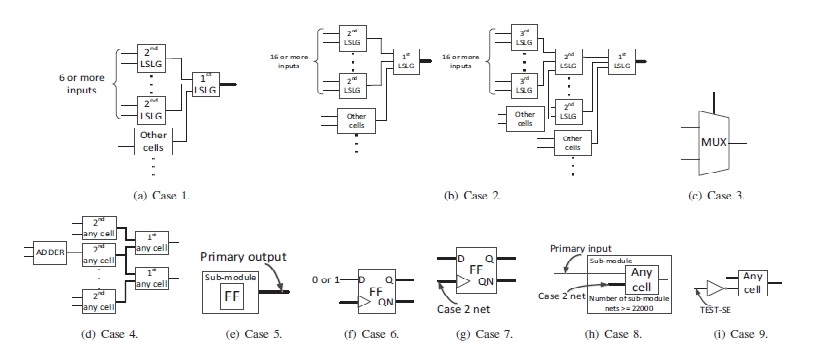
\includegraphics[width=\textwidth,keepaspectratio]{../pictures/hw_trojan_nets.jpg}
    \label{hw_trojans_nets}
    \caption{Register Transfer Level depiction of the proposed Hardware Trojan nets}
\end{figure}

The publication states, that trough the count of certain net types, the presence
of hardware trojans can be determined, but not their absence.
This insight leads to the assumption, that hardware design can be classified 
using the count of certain net types. 




